\documentclass{vgtc}                          % final (conference style)
%\documentclass[review]{vgtc}                 % review
%\documentclass[widereview]{vgtc}             % wide-spaced review
%\documentclass[preprint]{vgtc}               % preprint
%\documentclass[electronic]{vgtc}             % electronic version

\graphicspath{{figs/}}
\usepackage{times}
\renewcommand*\ttdefault{txtt}
\usepackage{mathptmx}
\usepackage{amsmath}

% Define \etal command
\newcommand{\etal}{\textit{et al.}}

% comment in following line for Japanese text
% \usepackage[whole]{bxcjkjatype}

\onlineid{0}
\vgtccategory{Research}
\vgtcinsertpkg
%\preprinttext{To appear in an IEEE VGTC sponsored conference.}
%\ieeedoi{xx.xxxx/TVCG.201x.xxxxxxx}

%% Paper title.

\title{Extending Voronoi Treemap-Based Text Visualization to Non-Convex Regions}

%% This is how authors are specified in the conference style

%% Author and Affiliation (single author).
%%\author{Roy G. Biv\thanks{e-mail: roy.g.biv@aol.com}}
%%\affiliation{\scriptsize Allied Widgets Research}

%% Author and Affiliation (multiple authors with single affiliations).
%%\author{Roy G. Biv\thanks{e-mail: roy.g.biv@aol.com} %
%%\and Ed Grimley\thanks{e-mail:ed.grimley@aol.com} %
%%\and Martha Stewart\thanks{e-mail:martha.stewart@marthastewart.com}}
%%\affiliation{\scriptsize Martha Stewart Enterprises \\ Microsoft Research}

%% Author and Affiliation (multiple authors with multiple affiliations)
\author{Naoya Oda \thanks{e-mail: oden6680@gmail.com}\\ \scriptsize Nihon University %
\and Yosuke Onoue \thanks{e-mail: onoue.yousuke@nihon-u.ac.jp}\\ \scriptsize Nihon University}

% \teaser{
%   \centering
%   \includegraphics[width=17cm]{teaser.pdf}
%   \caption{teaser image}
% }

\teaser{
  \centering
  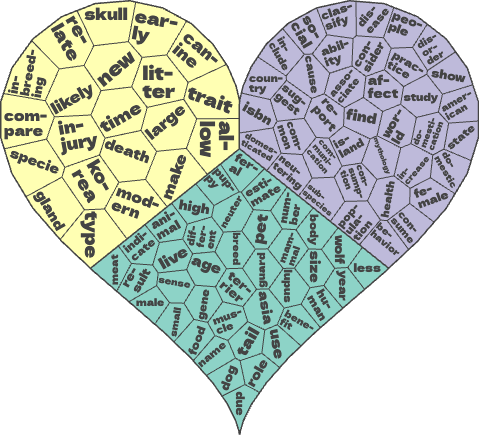
\includegraphics[width=0.45\textwidth]{figs/storygem_heart.png}
  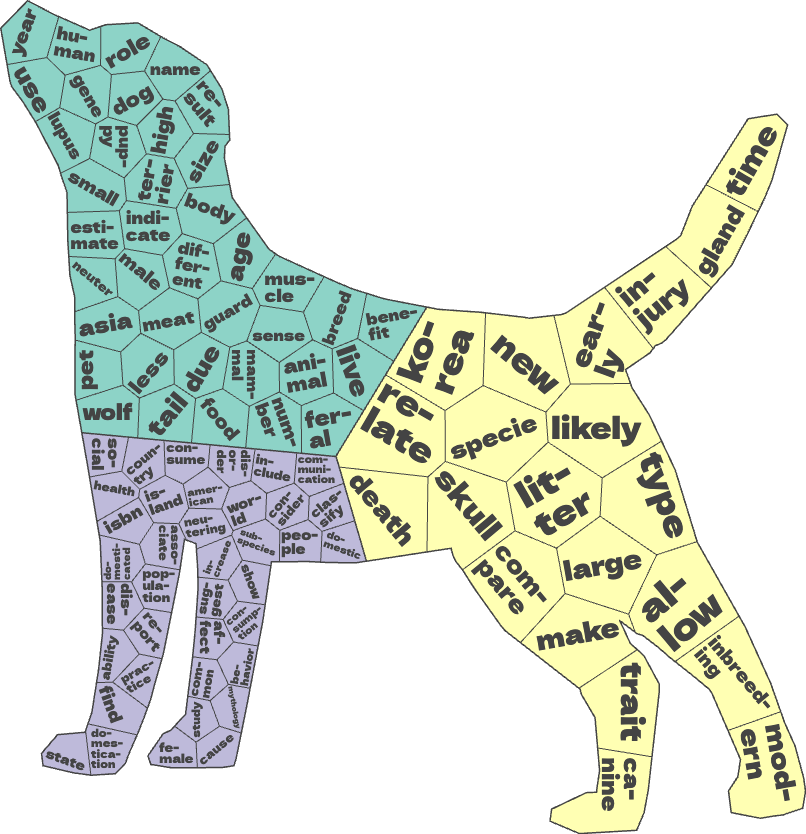
\includegraphics[width=0.45\textwidth]{figs/storygem_dog.png}
  \caption{
    Examples of StoryGem applied to non convex shapes using text from Wikipedia's Dog article: heart shaped region (left) and dog silhouette region (right). The method successfully fills these complex shapes while maintaining semantic relationships between dog related terms.
  }
  \label{fig:teaser}
}

\abstract{
  StoryGem is a text visualization technique that addresses WordCloud's inability to capture semantic connections and SemanticWordCloud's difficulty in efficiently filling defined areas.
  However, the original StoryGem is limited to convex regions.
  We present an extension that enables StoryGem to execute on non convex regions.
  This extension opens new possibilities for visualizations using geographical boundaries, corporate logos, and other meaningful shapes.
}

\CCScatlist{
  \CCScatTwelve{Human-centered computing}{Visualization}{Visualization application domains}{Information visualization}
  \CCScatTwelve{Human-centered computing}{Visualization}{Visualization techniques}{Treemaps}
}

% \nocopyrightspace

%%%%%%%%%%%%%%%%%%%%%%%%%%%%%%%%%%%%%%%%%%%%%%%%%%%%%%%%%%%%%%%%
%%%%%%%%%%%%%%%%%%%%%% START OF THE PAPER %%%%%%%%%%%%%%%%%%%%%%
%%%%%%%%%%%%%%%%%%%%%%%%%%%%%%%%%%%%%%%%%%%%%%%%%%%%%%%%%%%%%%%%%

\begin{document}
\firstsection{Introduction}
\maketitle

WordCloud\cite{viegas2009participatory} is a ubiquitous text visualization method that arranges words with varying sizes to represent importance.
However, traditional WordClouds use random layouts that fail to convey semantic relationships between words, limiting their analytical value for understanding text structure and meaning.
SemanticWordCloud\cite{wu2011semantic} and similar approaches attempt to preserve word relationships through spatial proximity but struggle with efficiently packing words into fixed areas.
This challenge becomes even more complex when dealing with non rectangular display regions.

Recent advances in text visualization have explored the use of arbitrary shapes for word layouts.
ShapeWordle~\cite{8807355} demonstrated the value of filling arbitrary shapes with words, showing that non convex region support has practical merit for creating visually engaging and contextually appropriate visualizations.
Building on these foundations, StoryGem~\cite{oda2025storygemvoronoitreemapapproach} introduced a novel approach using Voronoi treemaps to create continuous layouts where area encodes importance, avoiding the overemphasis of long words while preserving semantic relationships.
User studies confirmed that this approach helps viewers better understand text structure and identify related concepts.

However, StoryGem's font size optimization algorithm requires all Voronoi cells to be convex polygons, which restricts the method to convex display regions and limits its applicability to real world visualization scenarios.
Many practical applications require non convex shapes: geographic boundaries for regional text analysis, corporate logos for brand aligned visualizations, or thematically relevant shapes for educational materials.
The inability to handle such shapes significantly constrains StoryGem's utility in these contexts.

In this paper, we extend StoryGem to support arbitrary non convex domains through a novel font size optimization approach.
By computing convex hulls for individual Voronoi cells and applying binary search scaling, we preserve StoryGem's sophisticated optimization while enabling compatibility with complex shapes.
This advancement opens new visualization possibilities where the shape itself can reinforce the semantic content being displayed.

\section{Method}

We extend the original StoryGem framework to support non convex regions through three main stages with critical modifications.

\paragraph{Building a Semantic Word Network}
The preprocessing pipeline removes stop words and uses NLTK part of speech tagging to retain only verbs, nouns, and adjectives.
Word embeddings are extracted using a pretrained FastText model (157 languages, trained on CommonCrawl and Wikipedia), ensuring broad language coverage and semantic quality.
A $k$-nearest neighbor graph is constructed by computing cosine similarity between word pairs, creating a network that reflects semantic structure.
This network forms the foundation for subsequent clustering and layout operations.

\paragraph{Hierarchical Clustering and Voronoi Treemap Layout}
The Louvain method detects communities in the word network, creating reproducible hierarchical clusters that group semantically related terms.
These clusters are arranged using Balzer \etal's~\cite{balzer2005voronoi} Voronoi treemap algorithm, which performs iterative centroidal Voronoi tessellation.
This process allocates cell areas proportional to word weights (typically term frequency), creating a gapless layout that can fill non convex regions while maintaining area based importance encoding.
The key innovation is that this algorithm naturally handles non convex boundaries without modification.

\paragraph{Font Size Optimization for Non Convex Cells}
The original StoryGem's font size optimization requires all Voronoi cells to be convex polygons, which prevents its application to non convex regions.
Our key innovation is extending this optimization to work with non convex cells.
We compute the convex hull for each Voronoi cell and apply the original StoryGem's font size optimization algorithm to this convex hull.
However, since the optimized font size may cause text to extend beyond the actual non convex cell boundaries, we employ a binary search algorithm to scale down the font size until the text fits entirely within the cell.
This approach preserves the sophisticated optimization of the original StoryGem while ensuring compatibility with arbitrary cell shapes.
The binary search efficiently finds the maximum viable font size, maintaining both readability and aesthetic quality even in complex non convex regions.


\section{Application Examples}

To demonstrate the effectiveness of our non convex extension, we applied StoryGem to text data from Wikipedia's Dog article, visualizing it within a heart shape and a dog silhouette (Figure~\ref{fig:teaser}).
These shapes were specifically chosen to test the method's ability to handle both decorative and semantically meaningful non convex regions.

The heart shaped visualization tests our method's handling of smooth, curved boundaries combined with a sharp inward cusp.
The algorithm adapts gracefully to these varying geometric properties, filling the space completely while maintaining semantic coherence.
The smooth word distribution across curved boundaries demonstrates the method's versatility.

The dog silhouette visualization represents a significant advancement in practical applicability.
By successfully filling a complex dog shaped region with dog related terms from Wikipedia, we demonstrate that StoryGem can now handle semantically meaningful shapes that align with the content being visualized.
This capability enables intuitive, context aware visualizations where the shape reinforces the subject matter.
Successfully generating this visualization despite intricate contours (legs, tail, ears) proves our font size optimization handles highly complex non convex regions.

These examples reveal several key strengths of our extended StoryGem:
\begin{itemize}
  \item \textbf{Shape Flexibility}: The method successfully adapts to arbitrary non convex shapes without manual intervention or shape specific parameters
  \item \textbf{Semantic Preservation}: Hierarchical clustering and spatial proximity of semantically related words remain intact despite geometric constraints
  \item \textbf{Visual Quality}: Words are legibly sized and positioned, avoiding overlaps while maximizing space utilization
\end{itemize}

These results suggest numerous practical applications: geographic boundaries for regional text data, corporate logos for company terminology, and educational materials using meaningful shapes to enhance learning.

\section{Conclusions}

We have presented a significant extension of the StoryGem text visualization technique that removes the constraint of convex only display regions.
By developing a novel font size optimization approach that combines convex hull computation with binary search scaling, we enabled the application of StoryGem's sophisticated optimization to non convex cells.
This innovation allows meaningful text visualizations within arbitrary non convex shapes while preserving both the semantic relationships and the aesthetic quality that make StoryGem valuable.

Our experiments with heart shapes and dog silhouettes demonstrate that the method successfully handles both smooth curves and complex realistic shapes, maintaining semantic clustering even under challenging geometric constraints.
This opens new possibilities for contextually appropriate visualizations where the display shape can meaningfully relate to the content.

Non convex shape support has significant practical implications.
Geographic boundaries can visualize region specific text data within actual country, state, or district shapes.
Corporate logos can display company terminology in branded visualizations.
Educational materials can use meaningful shapes—brain for neuroscience terms, leaf for botanical vocabulary—creating memorable, context appropriate visualizations.

Several challenges remain for future work.
The current implementation requires predefined polygon shapes; a more flexible system would allow importing arbitrary shapes from image files and handling complex topologies with holes.
Extending to disconnected regions or shapes with internal voids would further broaden applicability.
Future work could explore more sophisticated text placement algorithms within non convex cells.

Despite these limitations, this extension of StoryGem represents a meaningful step toward more flexible and expressive text visualizations.
By enabling semantic word layouts within non convex shapes, we provide designers and analysts with new tools for creating visualizations that are both informative and visually aligned with their content's context.

\bibliographystyle{abbrv-doi}
\bibliography{reference}
\end{document}
